\chapter{Introduction}
\label{chap:intro}

% Also maybe add the benefits to network equipment vendors because of programmability.
%TODO: Diagram of smart end points and dumb routers
%TODO: Maybe diagrams of each of the three contributions?

Computer networks have two classes of elements: the \textit{end hosts} that
generate packets and the \textit{routers}\footnote{We use the term router to
refer to both routers and switches in this disseration.} that forward packets
between the end hosts. Traditionally, computer networks have followed the
end-to-end principle~\cite{e2e}: the principle that most of the
application-specific logic or intelligence in a network should reside at the
end hosts, while the routers themselves should be fixed-function devices
dedicated to forwarding packets as efficiently as possible. This dichotomy can
be seen in any popular Internet application today. Whether it is video
conferencing, web browsing, or social networking, each application's
distinctive application logic resides in clients and servers, while the routers
themselves just take care of forwarding packets between these clients and
servers. The end-to-end principle has in part been responsible for the dramatic
success and heterogeneity of the Internet because it allows applications to
implement their own logic at end hosts without touching the networks' routers.

Yet, today's reality is very different from the pristine network architecture
presented by the end-to-end principle. It is increasingly clear that routers
need to implement far more than packet forwarding. A typical router box today
implements features that far exceeds just packet forwarding, such as access
control, measurement support, and tunneling, because these are important to
network operators. A single router box today covers functionality that spans a
few 1000 RFCs~\cite{lavanya_compiler}. Yet, there's little consensus among
operators and vendors as to what goes features go into a router, and the
routers themselves are fixed-function. Inevitably, there are operators whose
needs fall outside the laundry list of features implemented by routers. In such
cases, the operator is out of luck because there is no way to modify a
fixed-function router to add a new feature that makese sense to a particular
operator.

We are reaching a point where the rate of innovation in new router algorithms
is outstripping our ability to get these algorithms into production routers.
Figure~\ref{fig:router_algos} shows a timeline of prominent router algorithms
that have been developed since the 1980s. Of these, only a handful are
available in production routers because there is no easy way to implement a new
router algorithm on a production router.

%TODO: What are production routers? Define them.
\begin{figure}
\centering
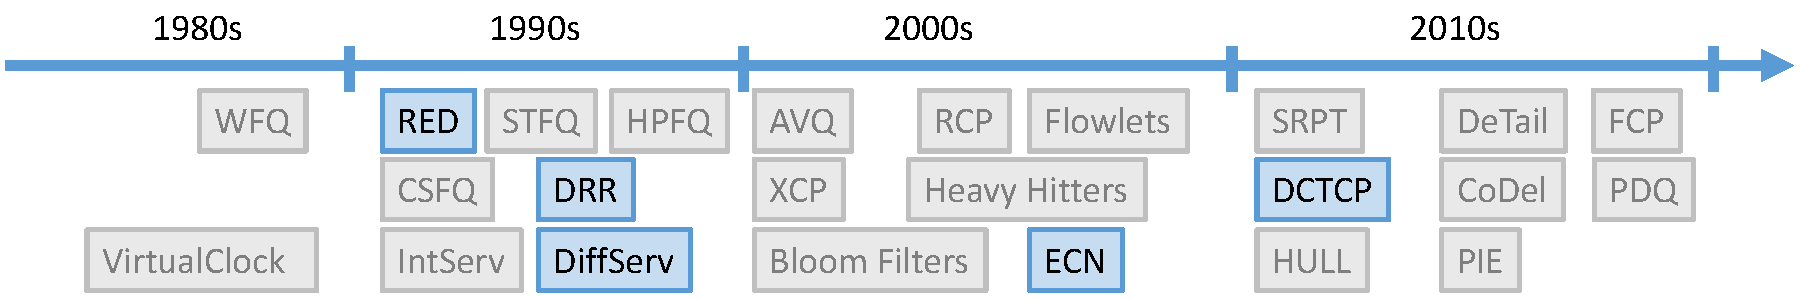
\includegraphics[width=\columnwidth]{router_alg_timeline.pdf}
\caption{Timeline of prominent router algorithms since the 1980s. Only the ones shaded in blue are available on production routers today.}
\label{fig:router_algos}
\end{figure}

As an operator who wants to implement some new functionality in a network, what
are the alternatives? One is to give up on changing routers altogether and make
all the required changes at the end hosts. But relying solely on end hosts
results in solutions that are cumbersome or suboptimal in many cases. As a
first example, imagine measuring the queuing latency at a particular hop in the
network by collecting end-to-end ping measurements between a variety of vantage
points and then fusing these measurements together to estimate per-hop queueing
latency. Not only is this indirect, it is also inaccurate relatively to just
instrumenting the router to measure it's own queueing latency. As a second
example, consider the problem of congestion control, which divides up a
network's capacity in some fair manner among competing users. There are many
in-network solutions to congestion control are superior in performance to the
end-host-only approaches to congestion control that are deployed today. Yet,
there is no way to deploy these in-network solutions today.

Another alternative for operators is to use a \textit{software router}: a
catch-all term for a router built on top of some \textit{programmable}
substrate, such as a general-purpose CPU, a network processor (a CPU with some
instructions tailored to packet processing), a GPU, or an FPGA. There are many
examples of such software routers~\cite{click, routebrucks, netfpga,
packetshader, ixp}. Figure~\ref{fig:router_evolution} tracks the aggregate
capacity of software routers over time and compares them against the fastest
routers known at a given point in time. The figure shows two trends. First, up
until the mid 90s, software routers were in fact the fastest routers; the early
routers were just minicomputers with special forwarding software. However,
since the mid 90s, growing demands for higher link speeds, fueled by the
Internet's explosive growth, have meant that the fastest routers tend to be
built out of dedicated hardware, specialized to packet forwarding. Further, the
performance of these routers is between 10 and 100 $\times$ more than software
routers. However, as we have been saying so far, these routers tend to
fixed-function as well and can not be programmed in the field unlike software
routers.

\begin{figure}
\centering
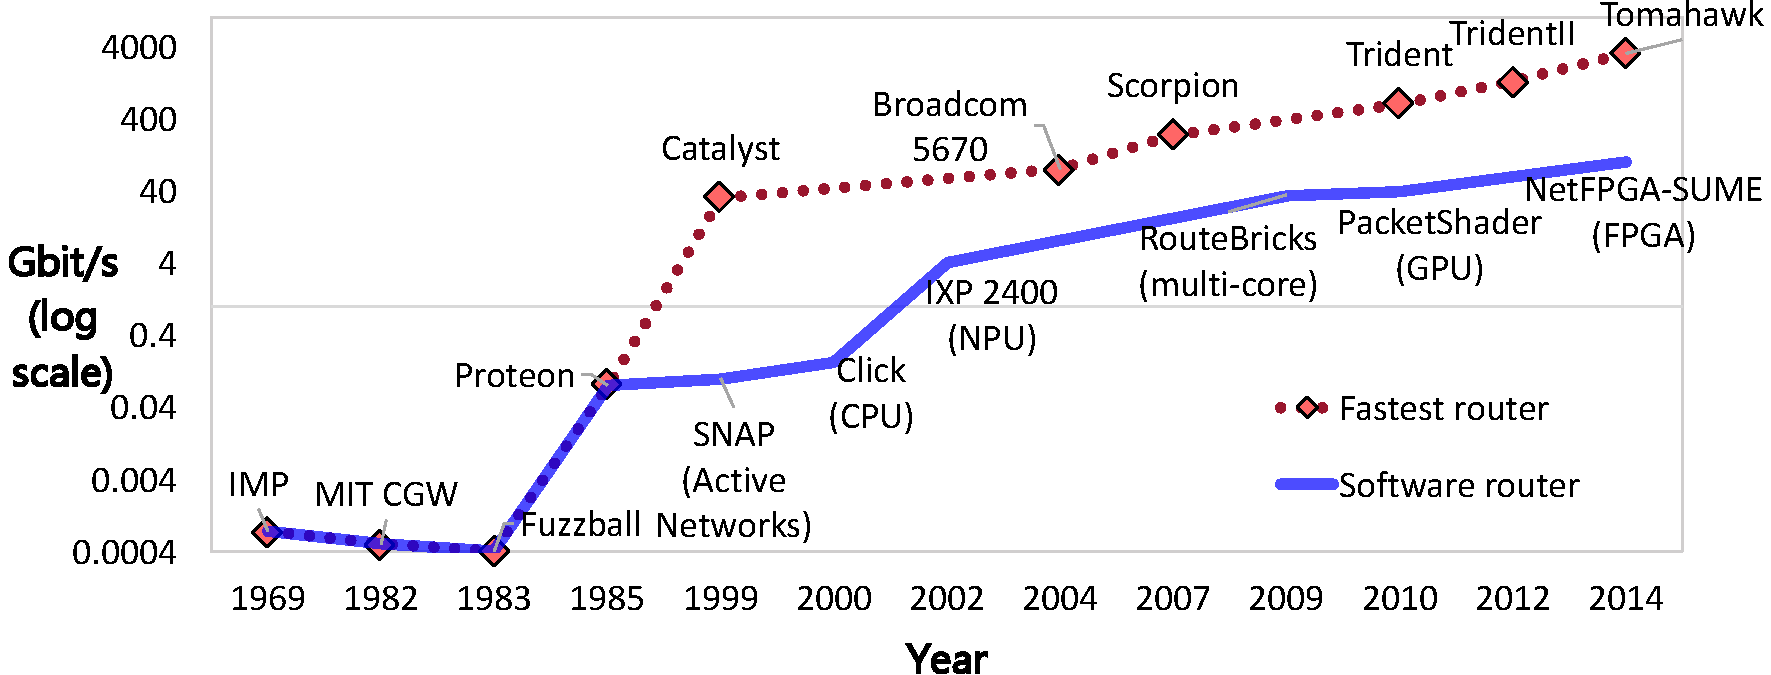
\includegraphics[width=\columnwidth]{router_evolution.pdf}
\caption{Aggregate capacity of routers since the first router on the ARPANET in
1969~\cite{imp}. Until the mid 90s, software routers were sufficient; since
then, however, the fastest routers have been built out of dedicated hardware.}
\label{fig:router_evolution}
\end{figure}


This dissertation considers the problem of building routers that are both fast
(\ie approaching the speed of the fastest fixed-function routers today), while
also being programmable. In particular, my thesis is that it is possible to
design router hardware that is both fast and programmable, as long as we
restrict ourselves to specific classes of router functionality. It is this
specificity that allows us to resolve this tension between programmability and
performance; indeed, the programmability provided by our designs is much more
restrictive than a Turing-complete processor. The challenge here is to pick
classes of router functionality that are actually practically useful to network
operators.

I will describe high-speed programmable hardware designs and their
corresponding programming models in software that target three classes of
router functionality.
\begin{CompactEnumerate}
\item Domino (\S\ref{chap:domino}) allows us to program \textit{streaming
algorithms} on high-speed router hardware. Streaming algorithms are algorithms
that operate on a sequeunce of packets, doing a bounded amount of work per
packet and manipulating a bounded amount of router state in the process. They
include algorithms for managing the router's buffer, load balancing, and
in-network congestion control.
\item Push-In First-Out Queues (\S\ref{chap:pifo}) allow us to program \textit{
scheduling algorithms}. These include classical schedulers such as Weighted
Fair Queueing~\cite{wfq}, Shortest Remaining Processing Time~\cite{srpt}, and
Hierarchical Packet Fair Queueing~\cite{hpfq}.
\item Performance Queries (\S\ref{chap:perf_query}) allow us to express a wide
variety of network performance measurement questions on high-speed router hardware. As an example, an operator could ask for a per-flow moving average of the
queueing latency on a particular network hop.
\end{CompactEnumerate}

%TODO: Do I need to describe the three contributions in more detail?
